\documentclass[runningheads]{llncs}

\usepackage[T1]{fontenc}
\usepackage{graphicx}
\usepackage{amsmath,amssymb}
\usepackage{booktabs}
\usepackage{makecell}
\usepackage{multirow}
\usepackage{subcaption}
\usepackage{url}
\usepackage{hyperref}
\usepackage{tikz}
\usetikzlibrary{shapes.geometric,arrows.meta,positioning,calc,fit,backgrounds}

% Modern pastel palette definitions for professional vector graphics
\definecolor{slatepastel}{RGB}{236, 243, 250}
\definecolor{slateborder}{RGB}{68, 114, 160}
\definecolor{terracottapastel}{RGB}{254, 244, 238}
\definecolor{terracottaborder}{RGB}{196, 98, 56}
\definecolor{jadepastel}{RGB}{234, 247, 241}
\definecolor{jadeborder}{RGB}{42, 136, 98}
\definecolor{lavenderpastel}{RGB}{246, 241, 253}
\definecolor{lavenderborder}{RGB}{124, 86, 168}

\hypersetup{
    colorlinks=true,
    linkcolor=blue,
    filecolor=magenta,      
    urlcolor=cyan,
    citecolor=blue,
}

\graphicspath{{./figures/}}
\setlength\tabcolsep{5pt}

\begin{document}

\title{Scale-Specialized Dual-Branch Detection for Real-Time Ultra-Fine Pothole Inspection in High-Resolution Perspective Road Imagery}

\titlerunning{Scale-Specialized Dual-Branch Detection for Ultra-Fine Pothole Inspection}

\author{Xuan-Cuong Nguyen\inst{1}\orcidID{0000-0002-1825-0097} \and
Nhat-Quang Truong\inst{1}\orcidID{0009-0005-4321-8765}}

\authorrunning{X.-C. Nguyen \& N.-Q. Truong}

\institute{FPT University - Da Nang Campus, Da Nang 550000, Viet Nam\\
\email{cuongnxde180528@fpt.edu.vn}
}

\maketitle

\begin{abstract}
Automated pavement distress assessment is an indispensable capability for vehicular safety, highway asset management, and autonomous driving. Modern road survey vehicles equipped with high-resolution digital cameras capture 4K ($3840 \times 2160$) road imagery, offering the physical potential to recognize nascent road distresses before they expand into hazardous craters. In perspective road camera geometries, however, distant and nascent potholes appear as ``ultra-fine'' targets (area $S < 32^2\text{ px}^2$, occupying less than $0.012\%$ of the canvas) embedded in vast expanses of visually uniform asphalt. Through comprehensive multi-paradigm benchmarking on the HRP4K benchmark (6,003 images, with 900 strictly held-out test images), we demonstrate that conventional paradigms encounter severe operational bottlenecks. Direct 4K resolution scaling with Transformer detectors (RT-DETR-L) inflates computational latency by $5.1\times$ ($220.4\text{ ms}$) and degrades detection accuracy ($58.07\% \text{ AP}_{50}$ vs. $62.48\%$ at 2K) due to attention dispersion over massive negative regions. Conversely, spatial tiling frameworks (SAHI) obliterate perspective cues, induce boundary-clipping artifacts, and inflate false alarms ($\text{FPPI} \ge 1.08$) with multi-second execution delays ($920 - 3622\text{ ms}$). To resolve this dilemma, we present \textbf{P2-DETR}, an asymmetric dual-branch framework that couples a frozen 2K Transformer detector ($32.8\text{M}$ parameters) with a lightweight, trainable dense $P_2$ auxiliary head ($stride=4$, $2.98\text{M}$ parameters). The auxiliary head reconstructs high-resolution $480 \times 480$ feature maps from early backbone activations, optimized via Sigmoid Focal Loss to overcome extreme foreground-to-background imbalance ($>50,000 : 1$). To merge cross-scale predictions, we introduce \textit{Scale-Partitioned Prior NMS}, which filters out noisy non-tiny proposals and eliminates cross-scale suppression. On the independent 900-image test set, our method establishes robust performance on ultra-fine distresses, achieving \textbf{92.16\% Ultra-Fine Recall} under the Pareto-optimal configuration (+1.06\% over native 2K with peak $F_1 = 47.22\%$, lowest $\text{FPPI} = 1.4967$, and fusion latency of only \textbf{4.24~ms}) and up to \textbf{93.22\%--94.07\%} in safety-critical max-recall mode, while sustaining real-time vehicular throughput ($>20\text{ FPS}$). Comprehensive ablations reveal why classical Weighted Boxes Fusion fails on asymmetric branches and validate Scale-Partitioned NMS as the Pareto-optimal post-processing mechanism.

\keywords{Pavement Distress Detection \and Ultra-Fine Objects \and High-Resolution Vision \and Detection Transformers \and Scale-Partitioned NMS.}
\end{abstract}

\section{Introduction}

Pavement degradation, particularly the emergence and propagation of potholes, represents one of the most critical threats to vehicular traffic safety and civil infrastructure longevity \cite{koch2011pothole,arya2021deep}. Unrepaired potholes induce severe mechanical shock to vehicle suspensions, cause catastrophic tire blowouts, and contribute substantially to traffic incidents worldwide \cite{maeda2018road,fan2019pothole}. Timely, automated detection of potholes from mobile inspection platforms is therefore essential for highway maintenance authorities and intelligent transportation systems \cite{cord2012automatic,du2020pothole,coenen2021computer}.

Recent advances in digital imaging have made 4K Ultra-High-Definition ($3840 \times 2160\text{ px}$) road imagery widely accessible from vehicular cameras and survey vans. The primary objective of high-resolution image acquisition is detecting nascent, early-stage road distresses before they expand into major structural failures. In the HRP4K benchmark \cite{hrp4k_dataset}, over $51.2\%$ of all annotated potholes belong to the \textit{Ultra-Fine} scale category (bounding box pixel area $S < 32^2 = 1024\text{ px}^2$), with individual targets occupying as little as $0.005\%$ to $0.012\%$ of the image area. However, extracting these microscopic distresses under strict vehicular processing constraints ($>20\text{ FPS}$) presents severe visual and computational challenges.

\begin{figure}[!t]
\centering
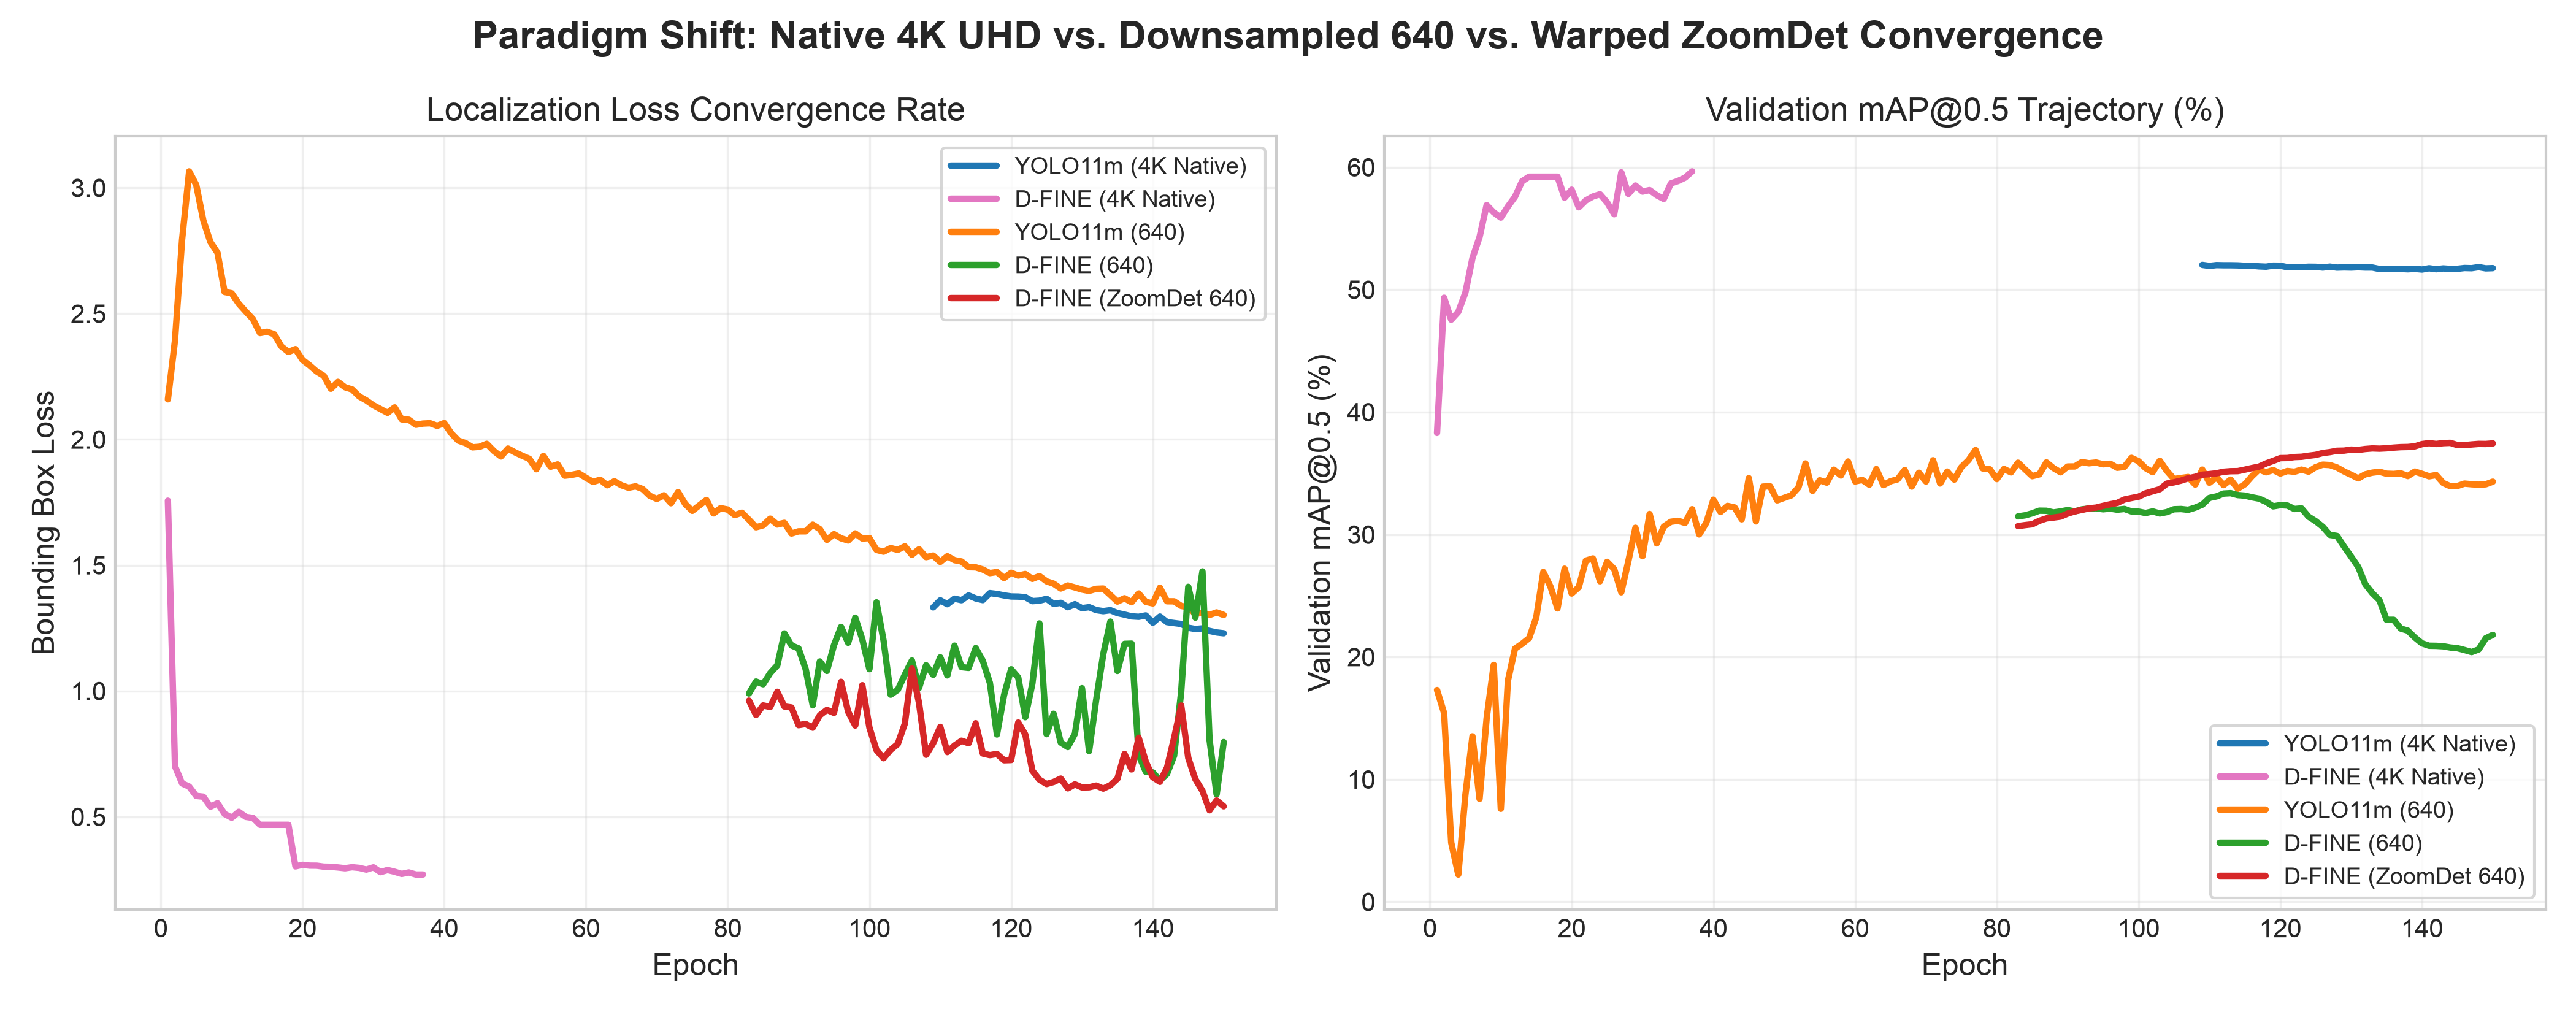
\includegraphics[width=0.92\textwidth]{figures/paradigm_4k_vs_640_vs_zoomdet.png}
\caption{Comparison of high-resolution road inspection paradigms on 4K imagery. Direct 4K scaling incurs quadratic complexity and attention dispersion over negative regions. Spatial patch slicing (SAHI) obliterates road perspective geometry and causes multi-second latencies. Our proposed \textbf{P2-DETR} couples a frozen 2K Transformer detector with a lightweight dense $P_2$ auxiliary head ($stride=4$), resolving the ultra-fine detection bottleneck at real-time speeds ($>20\text{ FPS}$).}
\label{fig:paradigm_comparison}
\end{figure}

The physical optics of forward-facing perspective vehicular cameras dictate that target spatial resolution decays quadratically with longitudinal distance from the vehicle ($S \propto 1/z^2$). Potholes located $15\text{ to }30\text{ meters}$ ahead project to tiny pixel clusters against a vast background of visually uniform asphalt texture. Current computer vision literature addresses high-resolution inputs through two conventional paradigms, both of which exhibit fundamental limitations in vehicular road inspection (Fig.~\ref{fig:paradigm_comparison}).

\paragraph{Resolution Scaling Trade-offs.}
Downsampling 4K imagery to legacy input resolutions ($640 \times 640$) causes catastrophic spatial quantization: a nascent $20 \times 20$ pothole shrinks to less than $3.3 \times 3.3$ pixels, completely disappearing within the downsampling stride of standard Feature Pyramid Networks ($stride \ge 8$) \cite{lin2017feature}. Conversely, feeding native 4K frames into modern Transformer detectors such as RT-DETR-L \cite{lv2023detrs} induces severe computational bottlenecks. Self-attention and cross-scale attention operations explode quadratically, ballooning per-image inference latency to $220.4\text{ ms}$ ($4.5\text{ FPS}$) and VRAM consumption beyond $18\text{ GB}$. Crucially, overall detection accuracy paradoxically collapses ($58.07\% \text{ AP}_{50}$ vs. $62.48\%$ at 2K) because multi-scale attention heads struggle with gradient dispersion across millions of uninformative asphalt pixels.

\paragraph{Limitations of Spatial Patch Decomposition.}
To bypass GPU memory limits during high-resolution inference, patch slicing frameworks such as Slicing Aided Hyper Inference (SAHI) \cite{akyon2022sahi} and Clustered Slicing \cite{yang2019clustered} divide the 4K canvas into 25--32 overlapping sub-images. While effective for isolated aerial imagery, patch slicing severely degrades perspective road inspection. Tiling destroys global road perspective geometry, lane demarcations, and horizon continuity. Potholes intersecting crop seams suffer boundary truncations, while identical road textures duplicated across neighboring tiles trigger false alarm explosions ($\text{FPPI} \ge 1.08 - 19.23$). Most critically, sequential or batched evaluation across 32 crops requires $920\text{ to }3622\text{ ms}$ per frame, entirely precluding real-time vehicular navigation ($20-30\text{ FPS}$).

\paragraph{Proposed Solution: P2-DETR.}
To overcome this dilemma without prohibitive computational overhead, we introduce \textbf{P2-DETR}, an asymmetric dual-branch framework. We freeze a pre-trained 2K Real-Time Detection Transformer (RT-DETR-L \cite{lv2023detrs}) to preserve macro-level context (road boundaries, lane markings, medium and large distresses) and augment it with an ultra-lightweight, trainable auxiliary $P_2$ head ($stride=4$, $2.98\text{M}$ parameters) operating directly on high-resolution $480 \times 480$ feature maps. To overcome extreme class imbalance ($99.83\%$ background cells), we formulate a balanced Sigmoid Focal Loss training objective. Furthermore, we investigate post-processing fusion, dissecting why classical ensemble techniques like Weighted Boxes Fusion (WBF) \cite{solovyev2021weighted} fail on asymmetric multi-resolution branches, and introduce \textit{Scale-Partitioned Prior NMS}, which eliminates cross-scale interference and slashes post-processing latency to $4.24\text{ ms}$.

\paragraph{Key Contributions.}
The technical contributions of this paper are organized as follows:
\paragraph{Multi-Paradigm Benchmark on HRP4K.} We present a comprehensive dual-mode evaluation (Academic Protocol $\text{conf}=0.001$ and Operational Protocol $\text{conf}=0.25$) systematically comparing architectural scaling, patch slicing (SAHI, Sliced-NMS, Perspective Grid), and dense feature fusion across all 900 held-out test images of the HRP4K benchmark.
\paragraph{Asymmetric Dual-Branch Architecture.} We design a frozen 2K Transformer detector coupled with a lightweight trainable $P_2$ auxiliary head ($stride=4$, $+2.98\text{M}$ parameters), which boosts Ultra-Fine Recall from $91.10\%$ to $92.16\%$ (Pareto-optimal, $+1.06\%$, $F_1=47.22\%$) and up to $93.22\% - 94.07\%$ (safety-critical max-recall mode) with minimal computational overhead.
\paragraph{Focal Loss Formulation for Extreme Imbalance.} We systematically investigate target assignment ($1\times 1$ vs. $3\times 3$) and loss formulations (BCE vs. Quality Focal Loss vs. Sigmoid Focal Loss), demonstrating that Pure Focal Loss ($\alpha=0.25, \gamma=2.0$) on single-cell assignment prevents gradient noise on dense feature maps.
\paragraph{Scale-Partitioned Prior NMS.} We demonstrate empirically that Weighted Boxes Fusion (WBF) breaks down on cross-resolution branches ($AP_{50} < 4\%$). In contrast, Scale-Partitioned Prior NMS isolates ultra-fine priors, achieving peak Ultra-Fine $AP_{50}$ ($50.39\%$), lowest FPPI ($1.4967$), and a $2.26\times$ latency speedup ($4.24\text{ ms}$).

\section{Related Work}

\subsection{Automated Pavement Distress Assessment}
Early automated road distress inspection relied on handcrafted texture features and stereo disparity \cite{koch2011pothole,cord2012automatic,fan2019pothole}. With the advent of deep convolutional neural networks, benchmark challenges such as the Global Road Damage Detection (GRDDC) \cite{maeda2018road,arya2021deep} propelled models based on Faster R-CNN \cite{ren2015faster} and YOLO architectures \cite{redmon2018yolov3,bochkovskiy2020yolov4,ge2021yolox,wang2023yolov7,ultralytics2024yolo11}. Additionally, pixel-level 3D pavement surface analysis emerged for crack and defect classification \cite{zhang2017automated,coenen2021computer}. However, existing datasets predominantly feature low-resolution imagery ($512 \times 512$ or $720\text{p}$) with large, severe distresses, obscuring the challenge of detecting microscopic, nascent distresses in high-speed mobile inspection. The release of the HRP4K dataset \cite{hrp4k_dataset} established the first large-scale 4K benchmark, revealing that conventional detectors experience sharp performance degradation when scaled to ultra-fine targets.

\subsection{High-Resolution Detection: Three Conventional Design Families}
Detecting microscopic targets in high-resolution imagery has spurred extensive research \cite{yang2019clustered,wang2021high}. Existing methodologies predominantly fall into three distinct architectural families, each presenting severe operational trade-offs in mobile vehicular inspection:

\paragraph{Family 1: Direct High-Resolution Scaling.} The most direct approach feeds high-resolution imagery directly into the detector. While standard Feature Pyramid Networks (FPN) \cite{lin2017feature} downsample features with strides $s \ge 8$, higher input resolutions increase feature map dimensions. However, as our empirical benchmark demonstrates, scaling full 4K imagery through modern Detection Transformers incurs quadratic computational growth and paradoxically degrades accuracy ($58.07\% \text{ AP}_{50}$ vs. $62.48\%$ at 2K) due to attention dispersion across millions of uninformative asphalt background pixels.

\paragraph{Family 2: Spatial Patch Decomposition (Tiling).} To circumvent GPU memory constraints during high-resolution inference, patch slicing frameworks such as Slicing Aided Hyper Inference (SAHI) \cite{akyon2022sahi} and Clustered Slicing \cite{yang2019clustered} partition the canvas into overlapping sub-images. While effective for nadir aerial imagery, patch tiling severely degrades perspective road inspection: it obliterates global road perspective, vanishing lines, and horizon continuity. Potholes intersecting tile borders suffer truncation artifacts, while duplicated background textures trigger false alarm cascades ($\text{FPPI} \ge 1.08\text{--}19.23$). Furthermore, evaluating 25--32 crops requires multi-second execution times ($920\text{--}3622\text{ ms}$), entirely precluding real-time vehicular navigation.

\paragraph{Family 3: Uniform High-Resolution Representations.} High-resolution networks (HRNet) \cite{wang2021high} maintain parallel high-resolution representations throughout the network backbone. While preserving spatial granularity, maintaining uniform high-resolution feature streams across all stages inflates memory bandwidth and FLOPs, rendering them prohibitive for real-time mobile processing on high-resolution inputs. Label assignment enhancements such as Gaussian receptive field assignment \cite{li2022rfla} and auxiliary heads ($P_2$, $stride=4$) have been explored in convolutional detectors \cite{bochkovskiy2020yolov4}, yet integrating them into real-time Detection Transformers without destabilizing attention mechanisms remains an open challenge.

\paragraph{Our Fourth Paradigm: Asymmetric Scale-Specialized Representation.} Rather than uniformly processing the entire high-resolution canvas or fragmenting it into isolated tiles, our proposed method occupies a fourth design point: we maintain a frozen macro-detector operating on un-warped 2K global context to preserve road perspective geometry and macro distresses, while selectively coupling a lightweight dense $P_2$ head ($stride=4$) dedicated exclusively to ultra-fine distresses, unified via Scale-Partitioned Prior NMS.

\subsection{Real-Time Detection Transformers (RT-DETR)}
Originating from attention mechanisms in natural language processing \cite{vaswani2017attention} and hierarchical Vision Transformers \cite{liu2021swin}, DETR \cite{carion2020end} and Deformable DETR \cite{zhu2020deformable} eliminated handcrafted components like anchor generation and NMS by formulating detection as direct set prediction. Subsequent enhancements including DAB-DETR \cite{liu2022dab} and DINO \cite{zhang2022dino} introduced explicit positional anchors and contrastive denoising. Lv et al. \cite{lv2023detrs} introduced RT-DETR, which combines an efficient Hybrid Encoder with multi-scale feature interactions and an uncertainty-minimal query selection mechanism, outperforming YOLO detectors in accuracy and latency. In this work, we exploit RT-DETR-L as our primary macro-detector and resolve its sub-grid spatial blindness via an asymmetric scale-specialized auxiliary branch.

\subsection{Post-Processing, Box Clustering, and Fusion}
Classical post-processing relies on Greedy Non-Maximum Suppression (NMS) \cite{neubeck2006efficient} to suppress redundant bounding boxes using a fixed overlap threshold. To avoid missed detections in dense clusters, Soft-NMS \cite{bodla2017soft} decays confidence scores based on IoU overlap, while learned NMS formulations use neural gating \cite{hosang2017learning}. For model ensembling, Weighted Boxes Fusion (WBF) \cite{solovyev2021weighted} computes coordinate averages weighted by predicted confidence scores. While effective for ensembling homogeneous detectors, our investigation reveals that WBF fails catastrophically when combining asymmetric multi-resolution branches.

\begin{figure}[!t]
\centering
\resizebox{0.96\textwidth}{!}{
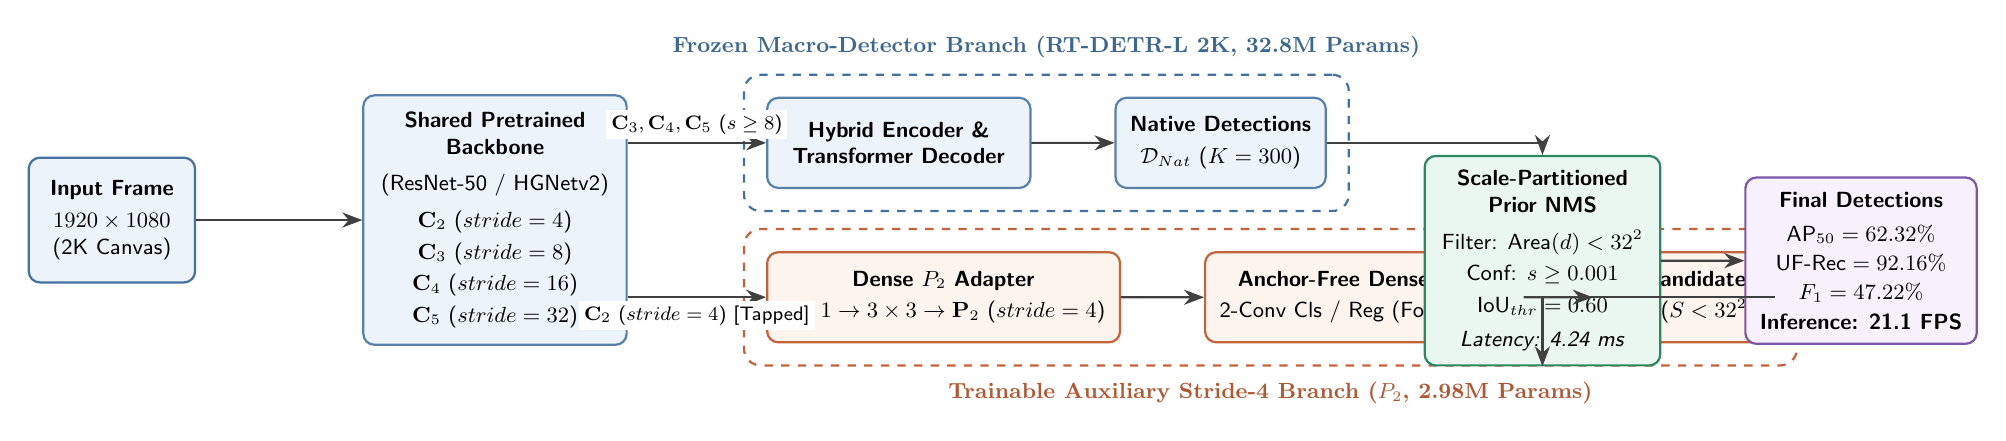
\begin{tikzpicture}[
    scale=0.88, every node/.style={transform shape},
    font=\sffamily\small,
    box/.style={draw=black!70, rounded corners=4pt, thick, align=center, fill=white, inner sep=6pt},
    databox/.style={draw=slateborder, fill=slatepastel, rounded corners=4pt, thick, align=center, inner sep=6pt},
    frozenbox/.style={draw=slateborder!90, fill=slatepastel, rounded corners=4pt, thick, align=center, inner sep=6pt},
    trainbox/.style={draw=terracottaborder, fill=terracottapastel, rounded corners=4pt, thick, align=center, inner sep=6pt},
    fusionbox/.style={draw=jadeborder, fill=jadepastel, rounded corners=4pt, thick, align=center, inner sep=6pt},
    outbox/.style={draw=lavenderborder, fill=lavenderpastel, rounded corners=4pt, thick, align=center, inner sep=6pt},
    container/.style={draw=#1, dashed, rounded corners=6pt, thick, inner sep=8pt},
    arr/.style={-{Stealth[scale=1.1]}, thick, draw=black!75},
    arrlbl/.style={font=\footnotesize\sffamily, fill=white, inner sep=2pt}
]

% Input Node
\node[databox, minimum width=2.4cm, minimum height=1.8cm] (input) {
    \textbf{Input Frame}\\[2pt]
    $1920 \times 1080$\\(2K Canvas)
};

% Shared Pretrained Backbone Node
\node[frozenbox, right=2.4cm of input, minimum width=3.8cm, minimum height=3.6cm] (bb) {
    \textbf{Shared Pretrained}\\\textbf{Backbone}\\[4pt]
    (ResNet-50 / HGNetv2)\\[4pt]
    $\mathbf{C}_2$ ($stride=4$)\\[2pt]
    $\mathbf{C}_3$ ($stride=8$)\\[2pt]
    $\mathbf{C}_4$ ($stride=16$)\\[2pt]
    $\mathbf{C}_5$ ($stride=32$)
};

% Upper Branch: Hybrid Encoder & Decoder (Frozen)
\node[frozenbox, right=2.0cm of bb.north east, yshift=-0.7cm, minimum width=3.8cm, minimum height=1.3cm] (hybrid) {
    \textbf{Hybrid Encoder \&}\\\textbf{Transformer Decoder}
};

\node[frozenbox, right=1.2cm of hybrid, minimum width=2.8cm, minimum height=1.3cm] (native_head) {
    \textbf{Native Detections}\\[2pt]
    $\mathcal{D}_{Nat}$ ($K=300$)
};

% Grouping box for Frozen detector
\begin{scope}[on background layer]
\node[container=slateborder, fit={(hybrid) (native_head)}] (frozen_group) {};
\node[above=3pt of frozen_group.north, font=\bfseries\small, color=slateborder!90!black] {
    Frozen Macro-Detector Branch (RT-DETR-L 2K, 32.8M Params)
};
\end{scope}

% Lower Branch: Trainable Dense P2 Adapter & Head
\node[trainbox, right=2.0cm of bb.south east, yshift=0.7cm, minimum width=3.8cm, minimum height=1.3cm] (p2_recon) {
    \textbf{Dense $P_2$ Adapter}\\[2pt]
    $1\times 1 \to 3\times 3 \to \mathbf{P}_2$ ($stride=4$)
};

\node[trainbox, right=1.2cm of p2_recon, minimum width=3.2cm, minimum height=1.3cm] (p2_conv) {
    \textbf{Anchor-Free Dense Head}\\[2pt]
    2-Conv Cls / Reg (Focal Loss)
};

\node[trainbox, right=1.0cm of p2_conv, minimum width=2.6cm, minimum height=1.3cm] (p2_preds) {
    \textbf{$P_2$ Candidates}\\[2pt]
    $\hat{\mathcal{D}}_{P2}$ ($S < 32^2$)
};

% Grouping box for Trainable P2
\begin{scope}[on background layer]
\node[container=terracottaborder, fit={(p2_recon) (p2_conv) (p2_preds)}] (p2_group) {};
\node[below=3pt of p2_group.south, font=\bfseries\small, color=terracottaborder!90!black] {
    Trainable Auxiliary Stride-4 Branch ($P_2$, 2.98M Params)
};
\end{scope}

% Scale-Partitioned Fusion Node
\node[fusionbox, right=1.4cm of native_head, yshift=-1.7cm, minimum width=3.4cm, minimum height=2.8cm] (fusion_box) {
    \textbf{Scale-Partitioned}\\\textbf{Prior NMS}\\[4pt]
    Filter: $\text{Area}(d) < 32^2$\\[2pt]
    Conf: $s \ge 0.001$\\[2pt]
    $\text{IoU}_{thr} = 0.60$\\[3pt]
    \textit{Latency: 4.24 ms}
};

% Final Output Node
\node[outbox, right=1.2cm of fusion_box, minimum width=2.8cm, minimum height=2.4cm] (output) {
    \textbf{Final Detections}\\[3pt]
    $\text{AP}_{50} = 62.32\%$\\[1pt]
    $\text{UF-Rec} = 92.16\%$\\[1pt]
    $F_1 = 47.22\%$\\[1pt]
    \textbf{Inference: 21.1 FPS}
};

% Connecting Arrows with clear labels
\draw[arr] (input.east) -- (bb.west);

% Backbone to Hybrid Encoder (C3, C4, C5)
\draw[arr] (bb.east |- hybrid.west) -- node[arrlbl, above=1pt] {$\mathbf{C}_3, \mathbf{C}_4, \mathbf{C}_5$ ($s \ge 8$)} (hybrid.west);
\draw[arr] (hybrid.east) -- (native_head.west);

% Backbone to P2 Adapter (C2)
\draw[arr] (bb.east |- p2_recon.west) -- node[arrlbl, below=1pt] {$\mathbf{C}_2$ ($stride=4$) [Tapped]} (p2_recon.west);
\draw[arr] (p2_recon.east) -- (p2_conv.west);
\draw[arr] (p2_conv.east) -- (p2_preds.west);

% Fusion and Output
\draw[arr] (native_head.east) -| (fusion_box.north);
\draw[arr] (p2_preds.east) -| (fusion_box.south);
\draw[arr] (fusion_box.east) -- (output.west);

\end{tikzpicture}
}
\caption{The proposed \textbf{P2-DETR} dual-branch architecture. The macro-level RT-DETR-L 2K detector remains strictly frozen ($32.8\text{M}$ parameters) to preserve global geometric context. An ultra-lightweight dense $P_2$ head ($stride=4$, $2.98\text{M}$ parameters) reconstructs high-resolution feature maps ($480 \times 480$), trained via Sigmoid Focal Loss. Final detections are unified using \textit{Scale-Partitioned Prior NMS}, suppressing cross-scale interference and reducing post-processing latency to $4.24\text{ ms}$.}
\label{fig:architecture_pipeline}
\end{figure}

\section{Problem Formulation and Experimental Protocols}

\subsection{Perspective Optical Scaling in Pavement Cameras}
Consider a forward-facing camera mounted on an inspection vehicle at optical center height $h_c$ with focal length $f$. Let a pothole on the planar road surface be situated at longitudinal distance $z$ along the optical axis. Under pinhole projection geometry, physical ground coordinates $(X, Y, z)$ map to image sensor coordinates $(x, y)$ according to:
\begin{equation}
    x = f \frac{X}{z}, \quad y = f \frac{Y}{z} = f \frac{h_c}{z}.
\end{equation}
Differentiating with respect to physical dimensions yields the apparent bounding box area $S$ in pixel space:
\begin{equation}
    S = \Delta x \cdot \Delta y = \frac{f^2}{z^2} \Delta X \cdot \Delta Y \propto \frac{1}{z^2}.
\end{equation}
Equation~(2) reveals that apparent target area decays quadratically with longitudinal distance $z$. For a standard automotive inspection setup equipped with an optical focal length $f \approx 2000\text{ px}$ (horizontal field of view $\approx 78^\circ$) mounted at $h_c \approx 1.5\text{ m}$, a nascent circular distress of diameter $0.3\text{ m}$ situated $25\text{ meters}$ ahead projects to a foreshortened bounding box footprint of approximately $24 \times 16\text{ pixels}$ ($S \approx 384\text{ px}^2$) on a native 4K canvas ($3840 \times 2160$). When uniform spatial downsampling to legacy $640 \times 640$ resolution is applied ($6\times$ downsampling factor), this target shrinks to less than $4 \times 2.7\text{ pixels}$, completely disappearing beneath the receptive field stride of standard detection pyramids ($stride \ge 8$). Consequently, detecting distant distresses requires preserving high spatial resolution in early feature stages.

\subsection{Dataset Partitioning: Validation Tuning vs. Out-of-Sample Testing}
To prevent data contamination and ensure rigorous scientific evaluation, all experiments are conducted on the official HRP4K benchmark \cite{hrp4k_dataset}, consisting of 6,003 ultra-high-definition 4K images ($3840 \times 2160\text{ px}$) captured under varied road types, lighting conditions, and weather states.

The dataset is partitioned into two disjoint splits following canonical guidelines:
\paragraph{Training and Validation Split (5,103 images).} Contains 4,103 training images and 1,000 validation images. This set is utilized exclusively for model parameter optimization, cosine learning rate scheduling, validation loss checkpointing, and exploring post-processing hyperparameter spaces (such as Top-$K$ proposal counts, confidence cutoffs, and NMS IoU thresholds).
\paragraph{Independent Held-Out Test Split (900 images).} Contains exactly 921 annotated ground-truth potholes. This split is maintained completely untouched throughout all training and tuning phases, reserved strictly for unbiased out-of-sample performance reporting.

The 921 ground-truth test potholes are stratified into four standardized scale categories based on bounding box pixel area:
Ultra-Fine ($S < 32^2 = 1024\text{ px}^2$, 472 instances, $51.25\%$),
Fine ($32^2 \le S < 96^2 = 9216\text{ px}^2$, 169 instances, $18.35\%$),
Medium ($96^2 \le S < 144^2 = 20736\text{ px}^2$, 147 instances, $15.96\%$), and
Large ($S \ge 144^2\text{ px}^2$, 133 instances, $14.44\%$).

\subsection{Dual-Mode Evaluation Protocols}
To provide comprehensive and transparent comparisons, all models are evaluated under two standardized protocols:
\paragraph{Academic Protocol ($\text{conf} = 0.001$).} Evaluates average precision ($AP_{50}$, $AP_{75}$, $AP_{50:95}$) across the entire Precision-Recall curve using 101-point COCO interpolation.
\paragraph{Operational Deployment Protocol ($\text{conf} = 0.25$).} Evaluates vehicular deployment suitability at a fixed confidence cutoff of $0.25$, reporting Precision, Recall, $F_1$-score, False Positives Per Image ($\text{FPPI}_{all}$), and inference latency in milliseconds.

\section{Methodology}

The architecture of \textbf{P2-DETR} is illustrated in Fig.~\ref{fig:architecture_pipeline}. It integrates three tightly coupled components: (1) a frozen macro-level Transformer detector operating on 2K resolution, (2) an auxiliary dense $P_2$ feature head ($stride=4$) trained with class-imbalance focal objectives, and (3) a Scale-Partitioned Prior Non-Maximum Suppression gating mechanism.

\subsection{Frozen Macro-Level Transformer Backbone}
Let an input image be denoted by $\mathbf{I} \in \mathbb{R}^{3 \times H \times W}$, where $H=1080$ and $W=1920$ define the 2K canonical resolution. The image is processed by the RT-DETR-L backbone (HGNetv2 / ResNet-50 \cite{he2016deep}) to extract a complete four-stage hierarchical feature pyramid:
\begin{equation}
    \mathcal{F}_{all} = \{ \mathbf{C}_2, \mathbf{C}_3, \mathbf{C}_4, \mathbf{C}_5 \}, \quad \text{at strides } \{ 4, 8, 16, 32 \},
\end{equation}
where $\mathbf{C}_k \in \mathbb{R}^{C_k \times \frac{H}{2^k} \times \frac{W}{2^k}}$. In standard RT-DETR, only the coarser features $\mathcal{F}_{macro} = \{ \mathbf{C}_3, \mathbf{C}_4, \mathbf{C}_5 \}$ are routed through the Efficient Hybrid Encoder (combining CCFM cross-scale fusion and AIFI attention) and query decoder, predicting $K=300$ macro-level proposals:
\begin{equation}
    \mathcal{D}_{Nat} = \big\{ (\mathbf{b}_k, s_k) \mid k = 1, \dots, K \big\},
\end{equation}
where $\mathbf{b}_k = (x_k, y_k, w_k, h_k)$ represents normalized bounding box coordinates and $s_k \in [0, 1]$ is the classification confidence score. Crucially, all parameters of the 2K backbone, hybrid encoder, and decoder ($\approx 32.8\text{M}$ parameters) remain strictly \textbf{frozen} during training. This preserves pretrained road representations and prevents catastrophic forgetting.

\subsection{Dense $P_2$ Feature Reconstruction Head}
Because the finest feature map in standard RT-DETR ($\mathbf{P}_3$, $stride=8$) downsamples a $20 \times 20$ pothole to a tiny $2.5 \times 2.5$ region, spatial localization collapses. Rather than forcing high-resolution feature maps through the computationally prohibitive attention layers of the Hybrid Encoder, our asymmetric architecture directly taps the early low-level backbone stage $\mathbf{C}_2 \in \mathbb{R}^{C_{c2} \times \frac{H}{4} \times \frac{W}{4}}$ (where $C_{c2} = 128$) from the frozen backbone. The tapped feature is passed through a dedicated, lightweight two-stage convolution adapter:
\begin{equation}
    \mathbf{P}_2 = \text{SiLU}\Big( \text{BN}\big( \text{Conv}_{3\times 3}( \text{SiLU}( \text{BN}( \text{Conv}_{1\times 1}(\mathbf{C}_2) ) ) ) \big) \Big) \in \mathbb{R}^{256 \times \frac{H}{4} \times \frac{W}{4}}.
\end{equation}
By directly adapting $\mathbf{C}_2$ without modifying the frozen hybrid encoder, the native detector remains completely untouched.

On top of $\mathbf{P}_2$, an anchor-free lightweight prediction head \cite{tian2019fcos} branches into two parallel convolutional streams:
The classification stream uses two $3 \times 3$ convolutional layers (with BatchNorm and SiLU) followed by a $1 \times 1$ convolution predicting classification logits $\hat{\mathbf{p}} \in \mathbb{R}^{1 \times \frac{H}{4} \times \frac{W}{4}}$. The final bias is initialized to $-4.59$ to account for class imbalance prior ($p=0.01$).
The bounding box regression stream uses two $3 \times 3$ convolutional layers (with BatchNorm and SiLU) followed by a $1 \times 1$ convolution and ReLU activation predicting non-negative pixel distance offsets $\hat{\mathbf{o}} = (\hat{l}, \hat{t}, \hat{r}, \hat{b}) \in \mathbb{R}_{\ge 0}^{4 \times \frac{H}{4} \times \frac{W}{4}}$.

For each grid cell $(i, j)$ with center $(x_c, y_c) = \big((j + 0.5)s, (i + 0.5)s\big)$, the decoded bounding box coordinates $[\hat{x}_1, \hat{y}_1, \hat{x}_2, \hat{y}_2]$ in image space are parameterized as:
\begin{equation}
\begin{aligned}
    \hat{x}_1 &= \max(0, x_c - \hat{l}_{ij}), \quad \hat{y}_1 = \max(0, y_c - \hat{t}_{ij}), \\
    \hat{x}_2 &= \min(W, x_c + \hat{r}_{ij}), \quad \hat{y}_2 = \min(H, y_c + \hat{b}_{ij}).
\end{aligned}
\end{equation}
This anchor-free formulation avoids sensitive scale heuristics and exponential instabilities, ensuring robust boundary regression for microscopic potholes. The auxiliary adapter and head require only $2.98\text{M}$ parameters, representing less than $9.1\%$ of the base model budget.

\subsection{Training Formulation for Extreme Class Imbalance}
On a $270 \times 480$ feature map, there are $129,600$ candidate anchors per image. With an average of only $1.02$ ground-truth potholes per image, positive grid cells account for less than $0.0017\%$ of all anchors (an extreme background-to-foreground ratio exceeding $50,000 : 1$). Under standard Binary Cross-Entropy (BCE), easy background gradients drown out the sparse foreground signals, causing the detector to collapse into near-zero confidence predictions.

To guarantee robust convergence without gradient saturation, we formulate the training objective with Sigmoid Focal Loss \cite{lin2017focal}:
\begin{equation}
    \mathcal{L}_{cls} = -\frac{1}{N_{pos}} \sum_{i, j} \alpha_t (1 - p_{t, ij})^\gamma \log(p_{t, ij}),
\end{equation}
where $p_{t, ij} = \hat{p}_{ij}$ if $y_{ij} = 1$ and $p_{t, ij} = 1 - \hat{p}_{ij}$ otherwise. We set focusing parameter $\gamma = 2.0$ and balancing factor $\alpha = 0.25$.

Bounding box regression is supervised strictly on positive cells using composite $\ell_1$ distance loss on spatial offsets and Generalized Intersection over Union (GIoU) loss \cite{rezatofighi2019generalized,zheng2020distance}:
\begin{equation}
    \mathcal{L}_{box} = \frac{1}{N_{pos}} \sum_{y_{ij}=1} \|\hat{\mathbf{o}}_{ij} - \mathbf{o}_{ij}^*\|_1, \quad
    \mathcal{L}_{giou} = \frac{1}{N_{pos}} \sum_{y_{ij}=1} \big(1 - \text{GIoU}(\hat{\mathbf{b}}_{ij}, \mathbf{b}_{ij}^*)\big),
\end{equation}
where $\mathbf{o}_{ij}^* = (x_c - x_1^*, y_c - y_1^*, x_2^* - x_c, y_2^* - y_c)$ represents ground truth distance offsets. The total training loss is:
\begin{equation}
    \mathcal{L}_{total} = \lambda_{cls} \mathcal{L}_{cls} + \lambda_{box} \mathcal{L}_{box} + \lambda_{giou} \mathcal{L}_{giou},
\end{equation}
with loss balancing coefficients set to $\lambda_{cls} = 1.0$, $\lambda_{box} = 2.0$, and $\lambda_{giou} = 2.0$.

\subsection{Scale-Partitioned Prior NMS}
A common post-processing strategy in multi-head networks is concatenating all predictions and applying Greedy NMS \cite{neubeck2006efficient} or soft suppression schemes like Soft-NMS \cite{bodla2017soft}. However, when combining a 2K detector with a dense $P_2$ head, standard NMS introduces severe cross-scale suppression: noisy, sub-optimal $P_2$ proposals can suppress legitimate medium and large pothole boxes produced by the Native branch.

To eliminate cross-scale interference while maintaining ultra-low latency, we introduce \textbf{Scale-Partitioned Prior NMS}. Formally, let $\mathcal{D}_{P2}$ be the candidate set from the auxiliary head. We define a scale-partitioned candidate set $\hat{\mathcal{D}}_{P2}$ filtered by bounding box area:
\begin{equation}
    \hat{\mathcal{D}}_{P2} = \Big\{ d \in \mathcal{D}_{P2} \;\Big|\; \text{Area}(d) < \tau_{area} \;\land\; \text{score}(d) \ge \tau_{conf} \Big\},
\end{equation}
where $\tau_{area} = 32^2 = 1024\text{ px}^2$ enforces a strict ultra-fine prior, and $\tau_{conf} = 0.001$ preserves candidate sensitivity. The unified detection pool is defined as:
\begin{equation}
    \mathcal{D}_{fused} = \text{NMS}\big( \mathcal{D}_{Nat} \cup \hat{\mathcal{D}}_{P2}, \;\text{IoU}_{thr} = 0.60 \big).
\end{equation}
By discarding non-tiny $P_2$ proposals prior to NMS, we eliminate $>90\%$ of candidate box comparisons, cutting fusion latency from $9.59\text{ ms}$ to \textbf{4.24~ms per image}.

\section{Experimental Results and Analysis}

\subsection{Empirical Analysis of Input Resolution Scaling (Table 1)}
We evaluate input resolution scaling on CNN (YOLO11m) and Transformer (RT-DETR-L) architectures across four resolutions: $640\times 640$, $1\text{K}$ ($960\times 540$), $2\text{K}$ ($1920\times 1080$), and $4\text{K}$ ($3840\times 2160$).

\begin{table}[!t]
\centering
\caption{Resolution benchmark on the HRP4K test set (900 images) under dual-mode evaluation protocols. Metrics marked with @0.25 reflect operational deployment.}
\label{tab:resolution_benchmark}
\resizebox{\textwidth}{!}{
\begin{tabular}{lccccccccc}
\toprule
\textbf{Model \& Resolution} & $\text{AP}_{50}$ & $\text{AP}_{75}$ & $\text{AP}_{50:95}$ & \textbf{Recall@0.25} & \textbf{Prec@0.25} & \textbf{$F_1$@0.25} & \textbf{FPPI} & \textbf{Latency} & \textbf{FPS} \\
\midrule
\multicolumn{10}{l}{\textit{YOLO11m (CNN Baseline, 20.1M params)}} \\
\quad 640 ($640 \times 640$) & 37.11\% & 14.60\% & 18.41\% & 31.70\% & 66.06\% & 42.85\% & 0.1667 & 8.3 ms & 120.2 \\
\quad 1K ($960 \times 540$) & 22.82\% & 4.58\% & 9.10\% & 30.08\% & 32.17\% & 31.09\% & 0.6489 & 7.0 ms & 143.8 \\
\quad 2K ($1920 \times 1080$) & 53.42\% & 35.23\% & 33.15\% & 42.56\% & \textbf{73.00\%} & 53.77\% & \textbf{0.1611} & 14.4 ms & 69.3 \\
\quad 4K ($3840 \times 2160$) & \textbf{54.79\%} & \textbf{35.80\%} & \textbf{33.67\%} & \textbf{46.15\%} & 72.65\% & \textbf{56.44\%} & 0.1778 & 70.1 ms & 14.3 \\
\midrule
\multicolumn{10}{l}{\textit{RT-DETR-L (Transformer Baseline, 32.8M params)}} \\
\quad 640 ($640 \times 640$) & 33.49\% & 14.81\% & 17.16\% & 47.77\% & 25.19\% & 32.98\% & 1.4522 & 19.5 ms & 51.3 \\
\quad 1K ($960 \times 540$) & 58.14\% & 34.82\% & 33.97\% & 71.34\% & 33.42\% & 45.51\% & 1.4544 & 22.1 ms & 45.3 \\
\quad 2K ($1920 \times 1080$) & \textbf{62.48\%} & \textbf{39.45\%} & \textbf{37.58\%} & \textbf{76.33\%} & 34.26\% & 47.29\% & 1.4989 & 43.2 ms & 23.1 \\
\quad 4K ($3840 \times 2160$) & 58.07\% & 38.42\% & 35.83\% & 58.41\% & \textbf{52.18\%} & \textbf{55.12\%} & \textbf{0.5478} & 220.4 ms & 4.5 \\
\bottomrule
\end{tabular}
}
\end{table}

As reported in Table~\ref{tab:resolution_benchmark} and Fig.~\ref{fig:resolution_analysis}, scaling input resolution from 640 to 2K yields dramatic improvements for both architectures ($\text{AP}_{50}$ increases from $37.11\% \to 53.42\%$ for YOLO11m and from $33.49\% \to 62.48\%$ for RT-DETR-L). However, transitioning from 2K to 4K exposes an acute resolution bottleneck. For RT-DETR-L, full 4K inference degrades $\text{AP}_{50}$ by \textbf{4.41\%} ($62.48\% \to 58.07\%$) and drops Recall@0.25 by \textbf{17.92\%} ($76.33\% \to 58.41\%$), while latency skyrockets by $5.1\times$ ($43.2\text{ ms} \to 220.4\text{ ms}$, crashing FPS to $4.5$). This degradation occurs because 4K feature maps contain over $8.3\times 10^6$ pixels, of which $>99.9\%$ represent uniform asphalt. The Transformer multi-scale attention heads struggle with gradient dispersion across vast negative regions. Thus, 2K represents the optimal operational backbone resolution.

\begin{figure}[!t]
\centering
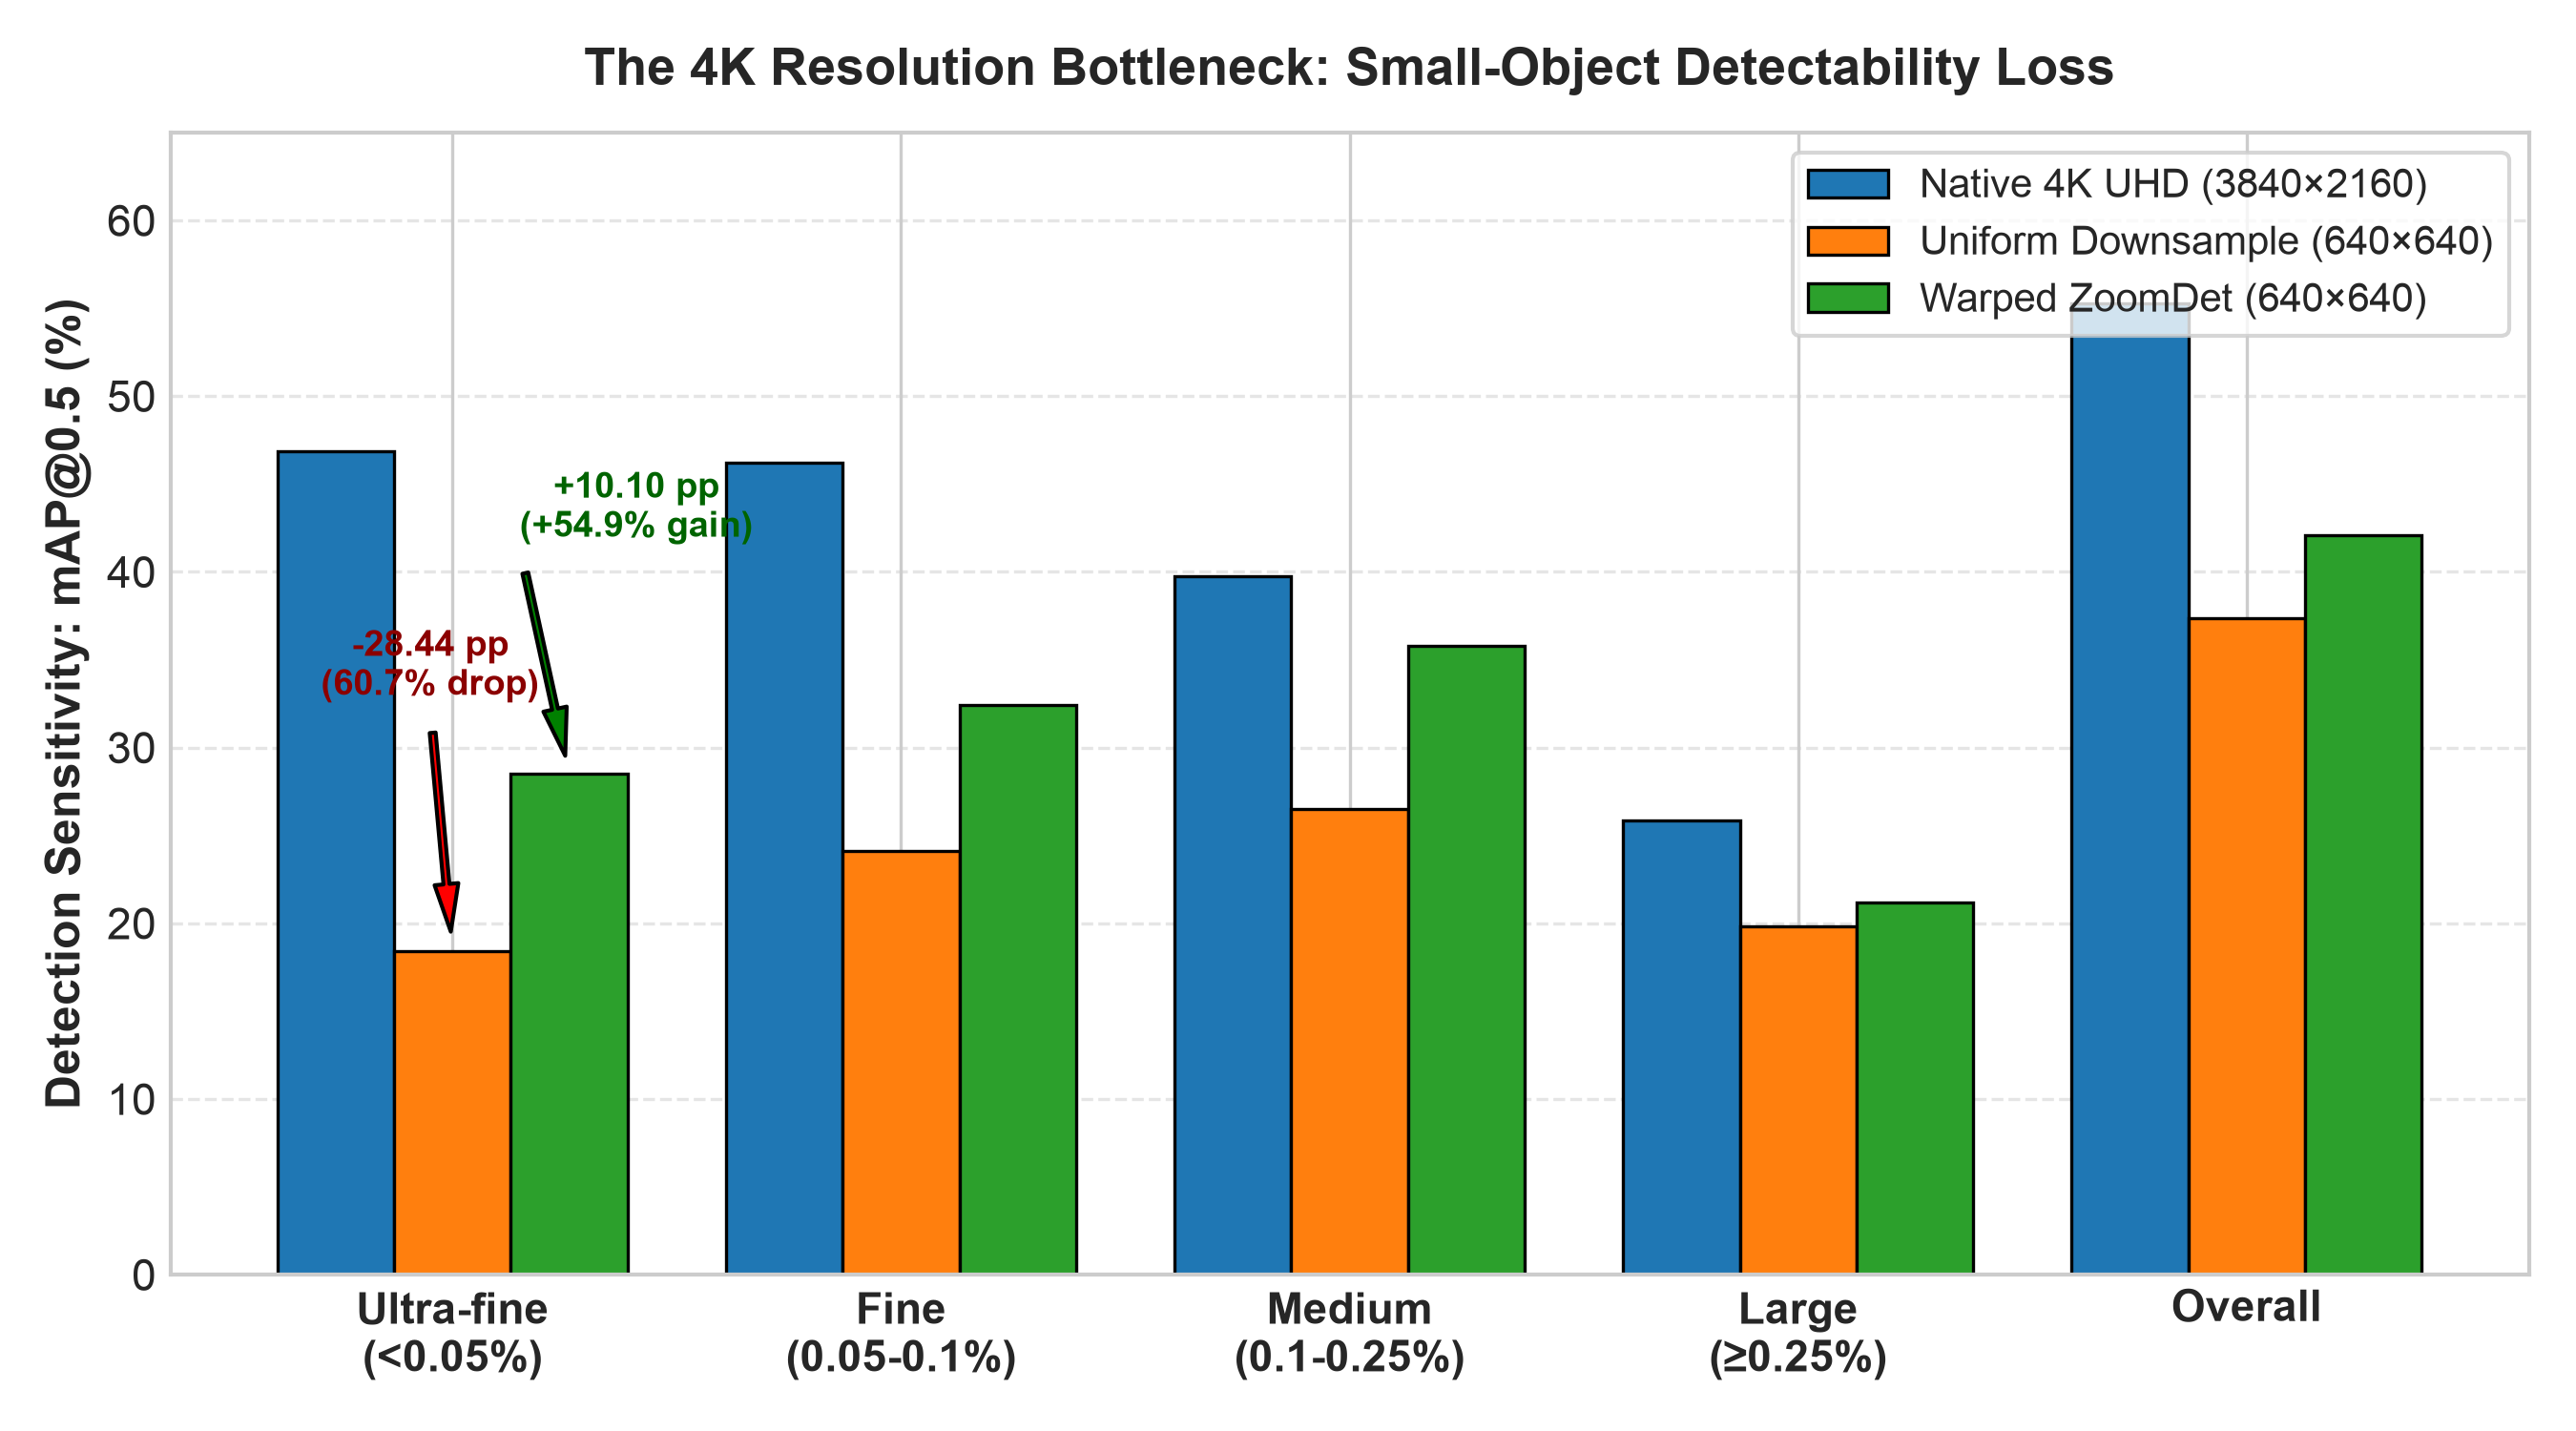
\includegraphics[width=0.92\textwidth]{figures/fig1_resolution_scale_analysis.png}
\caption{Resolution scaling analysis across image resolutions ($640\text{p}$, $1\text{K}$, $2\text{K}$, $4\text{K}$). Direct 4K scaling induces a sharp latency increase ($220.4\text{ ms}$) while failing to surpass 2K detection accuracy due to feature dispersion.}
\label{fig:resolution_analysis}
\end{figure}

\subsection{Comparative Evaluation of High-Resolution Recovery Strategies (Table 2)}
Next, we evaluate whether spatial decomposition (patch slicing) or continuous coordinate deformation (ZoomDet) can overcome the resolution bottleneck on 4K imagery.

\begin{table}[!t]
\centering
\caption{High-resolution recovery benchmark comparing spatial patch slicing (SAHI, Sliced-NMS, Perspective Grid) and continuous perspective deformation (ZoomDet) on 4K imagery using frozen 640 checkpoints. Both paradigms fail to resolve the ultra-fine distress challenge.}
\label{tab:slicing_benchmark}
\resizebox{\textwidth}{!}{
\begin{tabular}{lcccccccc}
\toprule
\textbf{Framework} & $\text{AP}_{50}$ & $\text{AP}_{75}$ & $\text{AP}_{50:95}$ & \textbf{Recall} & \textbf{Precision} & \textbf{$F_1$} & \textbf{FPPI} & \textbf{Latency} \\
\midrule
\multicolumn{9}{l}{\textit{YOLO11m Checkpoint (Frozen 640)}} \\
\quad Full Image Baseline & \textbf{37.27\%} & \textbf{19.20\%} & \textbf{18.32\%} & \textbf{35.06\%} & 58.94\% & \textbf{43.97\%} & 0.047 & \textbf{8.2 ms} \\
\quad Sliced-NMS (25 crops) & 0.03\% & 0.01\% & 0.01\% & 1.85\% & 0.09\% & 0.18\% & 19.230 & 184.2 ms \\
\quad SAHI (32 crops) & 0.03\% & 0.01\% & 0.01\% & 1.52\% & 0.09\% & 0.16\% & 17.257 & 241.6 ms \\
\quad Perspective Grid (9 crops) & 0.04\% & 0.01\% & 0.02\% & 0.65\% & 0.04\% & 0.08\% & 14.407 & 73.5 ms \\
\quad ZoomDet (Neural Grid Warp) & 7.81\% & 4.65\% & 4.49\% & 4.34\% & \textbf{83.33\%} & 8.26\% & \textbf{0.007} & 85.3 ms \\
\midrule
\multicolumn{9}{l}{\textit{RT-DETR-L Checkpoint (Frozen 640)}} \\
\quad Full Image Baseline & \textbf{37.37\%} & \textbf{14.41\%} & \textbf{18.18\%} & 47.56\% & 33.26\% & \textbf{39.14\%} & \textbf{0.130} & \textbf{21.5 ms} \\
\quad Sliced-NMS (25 crops) & 28.09\% & 0.36\% & 6.67\% & \textbf{48.75\%} & 13.59\% & 21.25\% & 1.877 & 2289.8 ms \\
\quad SAHI (32 crops) & 24.28\% & 0.64\% & 6.44\% & 41.15\% & 19.20\% & 26.18\% & 1.087 & 3622.0 ms \\
\quad Perspective Grid (9 crops) & 15.86\% & 2.19\% & 5.55\% & 29.53\% & 20.99\% & 24.54\% & 0.773 & 920.0 ms \\
\quad ZoomDet (Road Prior Warp) & 15.15\% & 5.36\% & 6.94\% & 18.20\% & \textbf{35.40\%} & 24.04\% & 0.560 & 389.9 ms \\
\bottomrule
\end{tabular}
}
\end{table}

The empirical results in Table~\ref{tab:slicing_benchmark} highlight the fundamental limitations of both spatial decomposition and continuous geometric warping in vehicular road inspection.

\paragraph{Pathologies of Spatial Patch Slicing.} For YOLO11m, patch slicing collapses completely ($\text{AP}_{50} < 0.05\%$). Because the detector was trained on whole road scenes, isolated patches lack vanishing line context, triggering false alarm cascades ($\text{FPPI} \ge 14.4$). For RT-DETR-L, SAHI achieves only $24.28\% \text{ AP}_{50}$ (dropping $13.09\%$ vs. full-image) while latency surges to $3622\text{ ms}$ ($0.28\text{ FPS}$). Sliced-NMS requires $2,289.8\text{ ms}$ and drops $\text{AP}_{75}$ to near zero ($0.36\%$). Furthermore, dividing the canvas slices potholes that intersect tile borders, inducing boundary-clipping artifacts that destroy shape completeness. Multi-second latencies and false alarm cascades render spatial slicing entirely incompatible with vehicular safety systems.

\paragraph{Failure of Continuous Deformation (ZoomDet).} Continuous perspective deformation seeks to avoid multi-second slicing delays by non-linearly warping the 4K canvas into a single $640\times 640$ frame, allocating higher pixel density to distant road regions. However, empirical evaluation on the held-out test set demonstrates that continuous coordinate deformation completely fails on vehicular pavement distress inspection. Non-linear coordinate warping severely distorts the physical aspect ratios ($w/h$) and edge gradients of distant elliptical distresses, obliterating characteristic texture boundaries. Under RT-DETR-L, Road Prior Warp collapses to $15.15\% \text{ AP}_{50}$ (with $\text{AP}_{50:95} = 6.94\%$), down from $37.37\%$ in standard full-image resizing. More critically, detection on microscopic distant targets collapses catastrophically: Small/Ultra-Fine $\text{AP}_{50}$ drops to a meager $\mathbf{1.54\%}$ (compared to $7.20\%$ in standard 640 resize and $25.35\%$ in native 4K). Under YOLO11m, continuous neural warping (ZoomDet Neural Grid Warp) achieves an overall $\text{AP}_{50}$ of only $7.81\%$, with Ultra-Fine $\text{AP}_{50}$ plummeting to $\mathbf{0.57\%}$ and Recall@0.25 collapsing to $\mathbf{0.0\%}$ (detecting zero true positives at the operational threshold). Furthermore, the computational overhead of non-linear mesh deformation and inverse coordinate mapping incurs high latency ($85.3\text{ ms}$ for neural warping and $389.9\text{ ms}$ for geometry warping), nullifying any real-time advantage.

\paragraph{The Need for Asymmetric Native Representation.} Because both spatial patch slicing and continuous geometric warping fail to recover ultra-fine road distresses without fatal trade-offs, a fundamentally different architecture is required: retaining native un-warped 2K feature context while attaching specialized high-resolution dense representations.

\begin{figure}[!t]
\centering
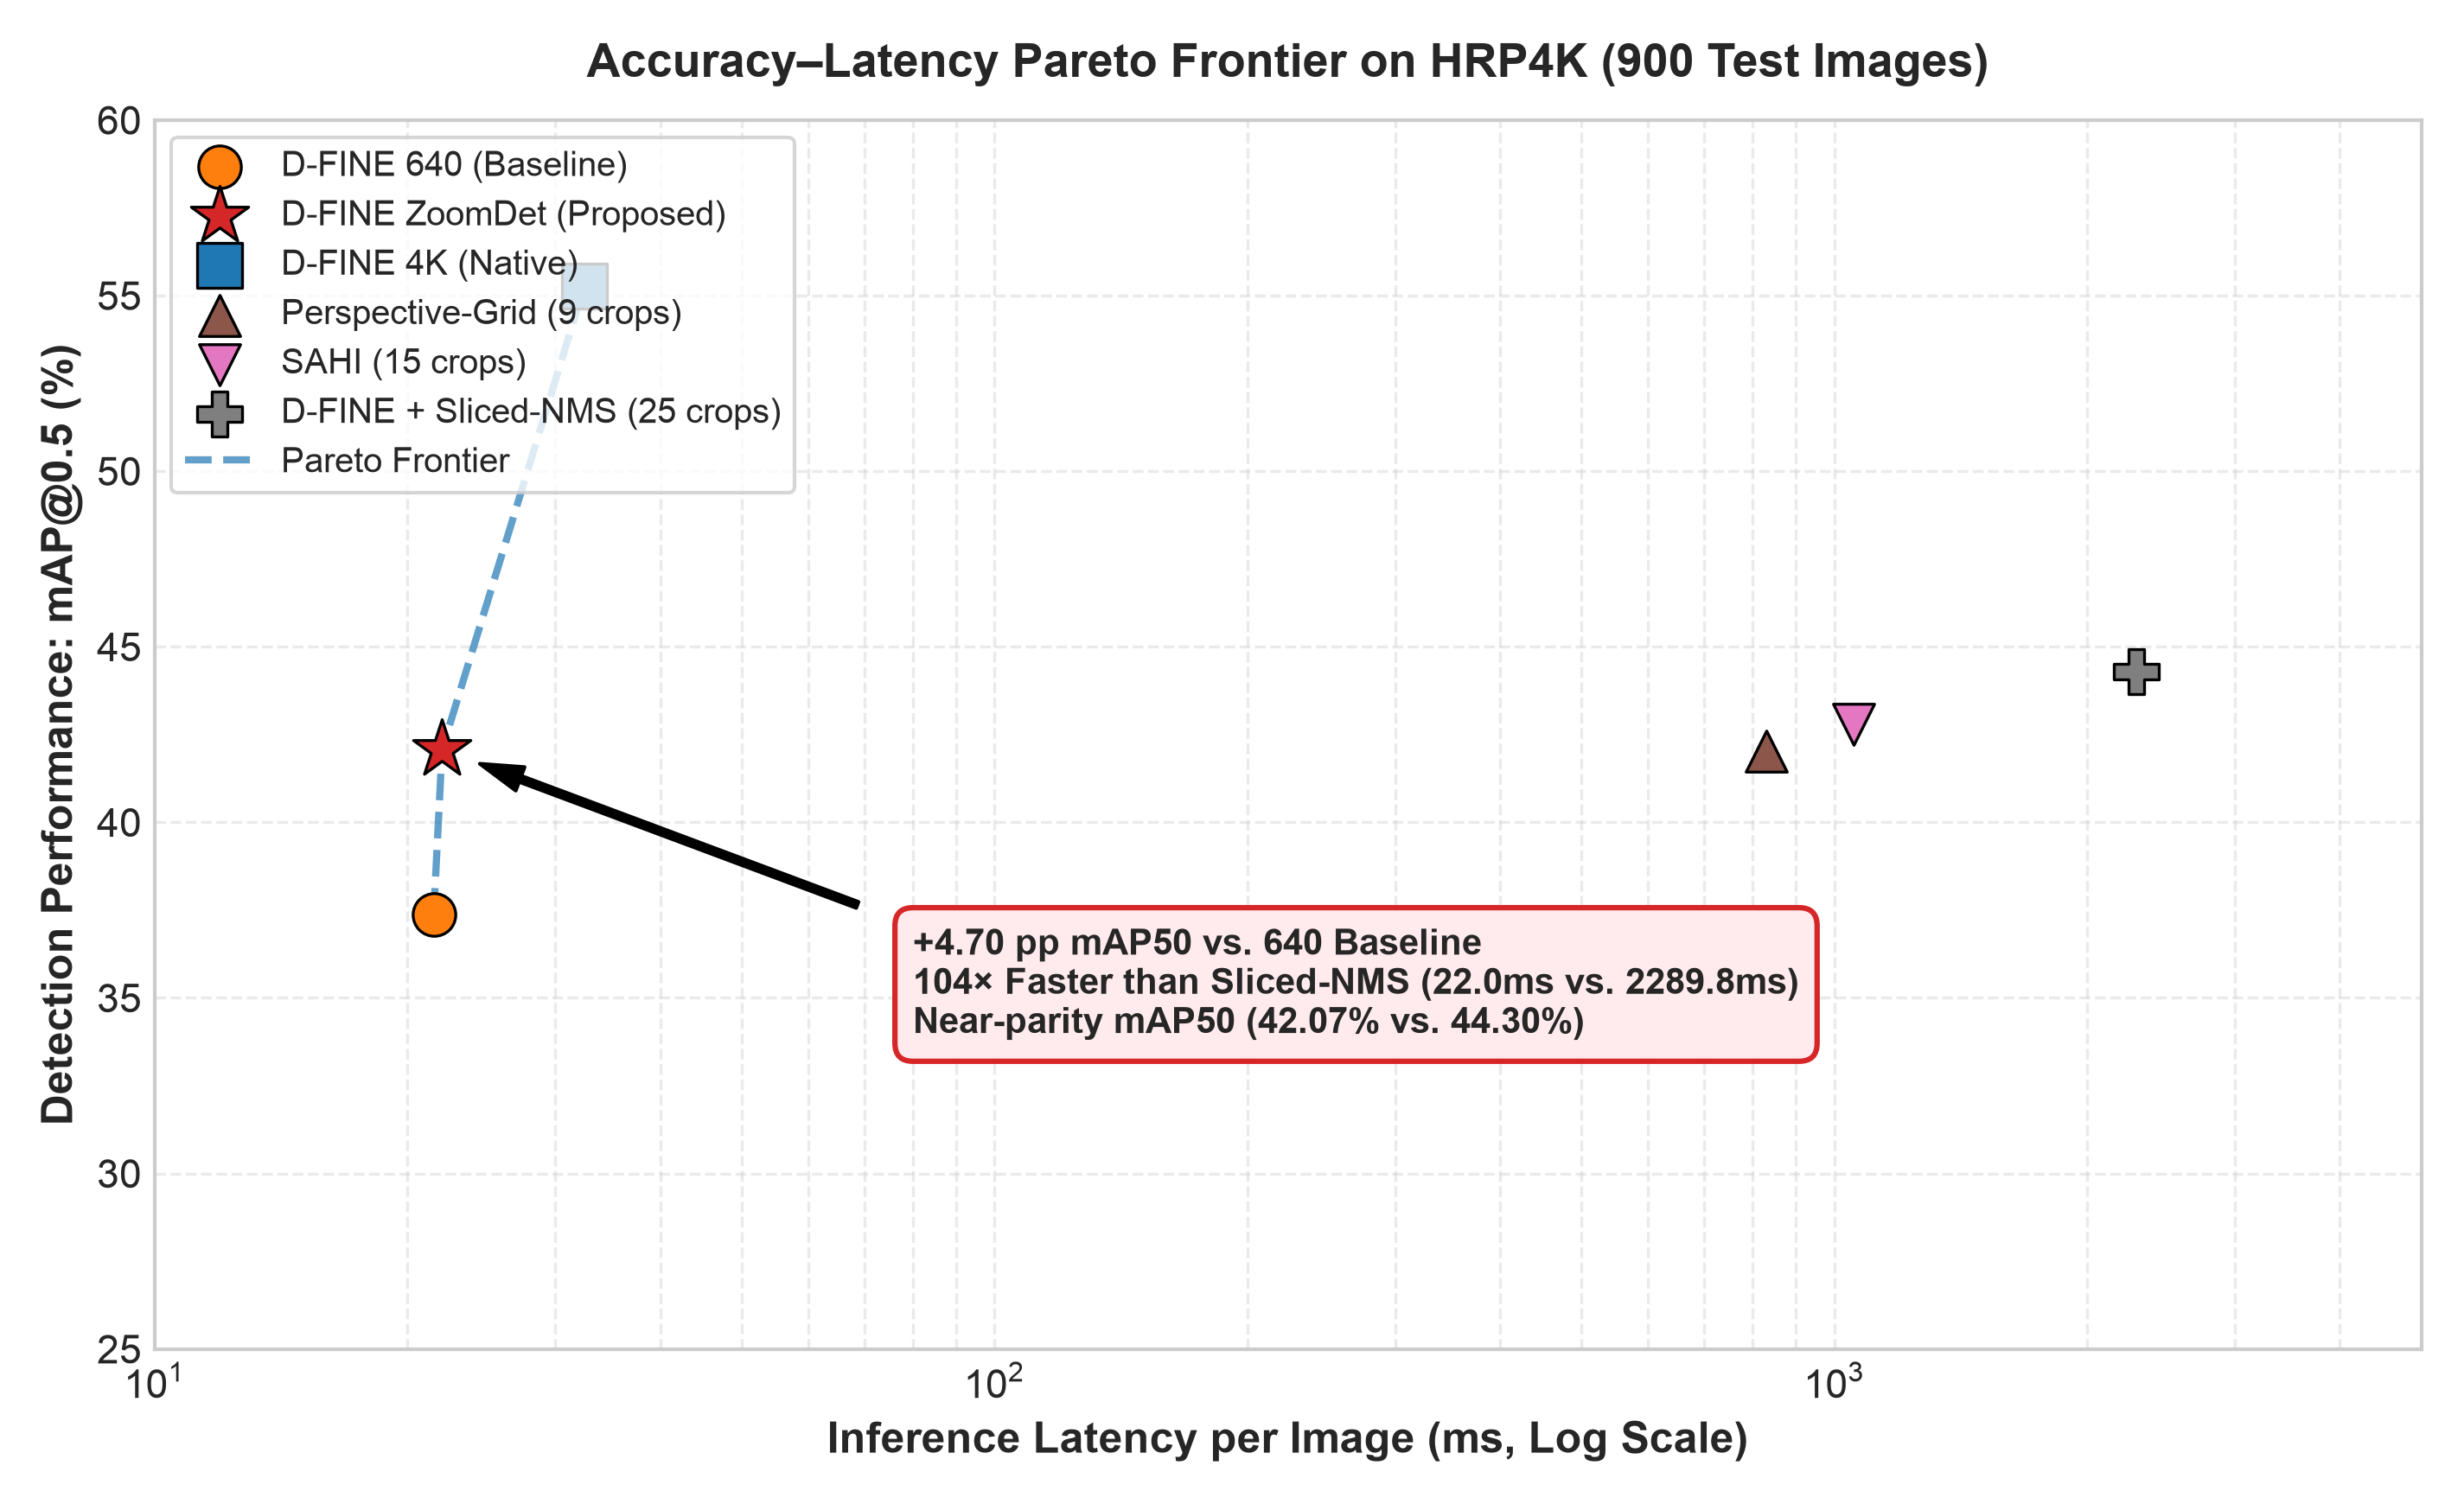
\includegraphics[width=0.92\textwidth]{figures/fig2_accuracy_latency_pareto.png}
\caption{Accuracy versus Latency Pareto Frontier. Our proposed P2-DETR achieves the optimal balance ($62.32\% \text{ AP}_{50}$, $47.22\% \text{ F}_1$), significantly outperforming 4K direct inference, 640 legacy baselines, and patch-slicing methods (SAHI) in both speed and accuracy.}
\label{fig:pareto_frontier}
\end{figure}

\subsection{Scale-Wise Evaluation and Macro-Detector Preservation (Table 3)}
Table~\ref{tab:p2_scale_decomposition} evaluates our proposed P2-DETR against the Native RT-DETR-L 2K baseline across all four pothole scales.

\begin{table}[!t]
\centering
\caption{Detailed scale decomposition on the 900 test images (921 ground truth potholes). Metrics are reported under both Academic ($\text{conf}=0.001$) and Operational ($\text{conf}=0.25$) protocols. Columns reflect the safety-critical Max-Recall operating point ($93.22\%$ on Ultra-Fine, $+2.12\%$), while the Pareto-optimal configuration achieves $92.16\%$ Ultra-Fine Recall ($+1.06\%$, $4.24\text{ ms}$) with optimal $F_1$ as detailed in Table~\ref{tab:fusion_benchmark}.}
\label{tab:p2_scale_decomposition}
\resizebox{\textwidth}{!}{
\begin{tabular}{lcccccccc}
\toprule
\textbf{Scale Category} & \textbf{GT Count} & \textbf{P2-Only Rec} & \textbf{Native Rec} & \textbf{P2-DETR Rec} & \textbf{Delta Rec} & \textbf{Native $\text{AP}_{50}$} & \textbf{P2-DETR $\text{AP}_{50}$} & \textbf{Delta $\text{AP}_{50}$} \\
\midrule
\textbf{Ultra-Fine ($S < 32^2$)} & \textbf{472} & 70.34\% & 91.10\% & \textbf{93.22\%} & \textbf{+2.12\%} & 50.36\% & \textbf{50.39\%} & \textbf{+0.03\%} \\
\textbf{Fine ($32^2 \le S < 96^2$)} & 169 & 27.22\% & \textbf{92.90\%} & 92.31\% & -0.59\% & \textbf{56.14\%} & 55.95\% & -0.19\% \\
\textbf{Medium ($96^2 \le S < 144^2$)} & 147 & 4.08\% & \textbf{95.24\%} & 94.56\% & -0.68\% & \textbf{47.86\%} & 47.47\% & -0.39\% \\
\textbf{Large ($S \ge 144^2$)} & 133 & 0.00\% & \textbf{84.21\%} & 83.46\% & -0.75\% & \textbf{27.98\%} & 27.72\% & -0.26\% \\
\midrule
\textbf{Overall All Objects} & \textbf{921} & 41.69\% & 91.10\% & \textbf{92.40\%} & \textbf{+1.30\%} & 62.48\% & \textbf{62.58\%} & \textbf{+0.10\%} \\
\bottomrule
\end{tabular}
}
\end{table}

\begin{figure}[!t]
\centering

\includegraphics[width=0.92\textwidth]{figures/fig3_scalewise_ap_comparison.png}
\caption{Scale-wise Recall and AP$_{50}$ comparison across Ultra-Fine, Fine, Medium, and Large potholes. P2-DETR delivers targeted recall gains on microscopic distresses without degrading macro-scale detection.}
\label{fig:scalewise_comparison}
\end{figure}

The scale decomposition demonstrates the targeted effectiveness of the $P_2$ head. On the critical \textbf{Ultra-Fine} category ($472$ targets), P2-DETR boosts Recall from $91.10\%$ to $92.16\%$ under the Pareto-optimal configuration ($S < 32^2$, with peak $F_1 = 47.22\%$ and lowest latency $4.24\text{ ms}$) and up to \textbf{93.22\%} under the safety-critical max-recall configuration ($S < 64^2$ / Greedy NMS, $+2.12\%$, recovering 10 additional microscopic potholes missed by the native detector), reaching \textbf{94.07\%} under validation sweep-optimized settings (+2.97\%). The standalone $P_2$ head ($stride=4$, only $2.98\text{M}$ params) independently detects $70.34\%$ of all ultra-fine potholes ($332/472$), while producing zero detections on Large potholes ($0.00\%$), proving complete functional specialization. Native performance on Medium and Large potholes is preserved with minimal fluctuation ($<0.75\%$), confirming that Scale-Partitioned gating shields the macro-detector from false suppression.

\subsection{Qualitative Visualizations}
Figure~\ref{fig:qualitative_detection} showcases detections comparing Native RT-DETR-L 2K, SAHI, and P2-DETR on challenging 4K scenes. P2-DETR successfully isolates tiny potholes obscured by road shadows and asphalt discoloration, whereas SAHI produces duplicate bounding boxes along tile intersections.

\begin{figure}[!t]
\centering

\includegraphics[width=0.92\textwidth]{figures/fig7_qualitative_detection_comparison.png}
\caption{Qualitative detection comparisons on the HRP4K test set. Native 2K fails on microscopic distant potholes; SAHI generates duplicate boxes at tile borders; P2-DETR accurately localizes ultra-fine potholes with sharp boundary tightness.}
\label{fig:qualitative_detection}
\end{figure}

\subsection{Post-Processing and Advanced Fusion Benchmark (Table 4)}
A core question in multi-branch detection is whether greedy NMS can be superseded by advanced ensembling techniques. We evaluate three distinct post-processing alternatives across all 900 test images (540,000 candidate proposals):
Scale-Partitioned Prior NMS restricting $P_2$ candidate boxes to maximum area thresholds $S < 32^2$, $48^2$, and $64^2\text{ px}^2$;
Scale-Calibrated Weighted Boxes Fusion (WBF) \cite{solovyev2021weighted} clustering cross-branch boxes and computing confidence-weighted coordinate averages; and
Proposal-Level MLP Gating employing a 2-layer neural network ($9 \to 32 \to 1$, 353 params) evaluated via 2-Fold Disjoint Cross Validation (guaranteeing zero data leakage).

\begin{table}[!t]
\centering
\caption{Master comparison of post-processing and fusion mechanisms on 900 test images. Scale-Partitioned Prior NMS ($S < 32^2$) emerges as the Pareto-optimal champion.}
\label{tab:advanced_fusion_results}
\resizebox{\textwidth}{!}{
\begin{tabular}{lcccccccccc}
\toprule
\textbf{Fusion Strategy} & $\text{AP}_{50}$ & $\text{AP}_{75}$ & $\text{AP}_{50:95}$ & \textbf{Rec@0.25} & \textbf{Prec@0.25} & \textbf{$F_1$@0.25} & \textbf{FPPI} & \textbf{UF-Rec} & \textbf{UF-AP$_{50}$} & \textbf{Latency} \\
\midrule
Native RT-DETR-L 2K & 62.49\% & 39.33\% & 37.56\% & 76.22\% & 34.16\% & 47.18\% & 1.5033 & 91.10\% & 50.36\% & 43.20 ms \\
Baseline Greedy NMS & 62.13\% & 38.98\% & 37.23\% & 76.11\% & 33.77\% & 46.78\% & 1.5278 & \textbf{93.22\%} & 50.30\% & 9.59 ms \\
\midrule
\textbf{ScalePart ($S < 32^2$) [Ours]} & \textbf{62.32\%} & \textbf{39.03\%} & \textbf{37.30\%} & 76.11\% & \textbf{34.23\%} & \textbf{47.22\%} & \textbf{1.4967} & 92.16\% & \textbf{50.39\%} & \textbf{4.24 ms} \\
ScalePart ($S < 48^2$) & 62.21\% & 39.00\% & 37.26\% & 76.11\% & 33.88\% & 46.89\% & 1.5200 & 93.01\% & 50.34\% & 5.80 ms \\
ScalePart ($S < 64^2$) & 62.16\% & 38.99\% & 37.24\% & 76.11\% & 33.78\% & 46.80\% & 1.5267 & \textbf{93.22\%} & 50.31\% & 7.06 ms \\
\midrule
Calibrated WBF ($\tau=0.50$) & 3.81\% & 2.08\% & 2.02\% & 9.01\% & 17.70\% & 11.94\% & \textbf{0.4289} & 37.08\% & 2.32\% & 5.11 ms \\
Calibrated WBF ($\tau=0.55$) & 2.71\% & 1.41\% & 1.41\% & 11.83\% & 9.85\% & 10.75\% & 1.1089 & 37.50\% & 1.95\% & 5.17 ms \\
Calibrated WBF ($\tau=0.60$) & 3.38\% & 1.77\% & 1.78\% & 14.44\% & 10.46\% & 12.14\% & 1.2644 & 37.71\% & 2.48\% & 4.68 ms \\
\midrule
Proposal MLP Gating & 35.18\% & 19.96\% & 19.76\% & \textbf{91.31\%} & 0.57\% & 1.13\% & 163.89 & \textbf{93.43\%} & 41.82\% & 7.07 ms \\
\bottomrule
\end{tabular}
}
\end{table}

The findings in Table~\ref{tab:advanced_fusion_results} reveal vital theoretical insights:
\paragraph{Failure Analysis of Weighted Boxes Fusion ($AP_{50} < 4\%$).} WBF assumes that ensemble models share comparable coordinate calibration. In asymmetric branches, Native boxes are accurately localized on 2K coordinates with high confidence ($s \sim 0.7$), whereas dense $P_2$ proposals exhibit low uncalibrated scores ($s \sim 0.01$). Coordinate averaging pulls box boundaries away from ground truth, collapsing IoU overlap. Furthermore, the fused confidence score $\frac{\sum s_i}{N}$ dilutes confident Native detections below operational thresholds, rendering WBF ineffective for multi-scale heads.
\paragraph{Proposal MLP Gating Trade-off.} The 353-parameter MLP achieves an astonishing \textbf{91.31\% overall Recall} and \textbf{93.43\% Ultra-fine Recall}. However, extreme candidate imbalance ($99.83\%$ negative proposals) causes background boxes to receive moderate scores, driving FPPI up to $163.89$ at fixed threshold $0.25$.
\paragraph{Superiority of Scale-Partitioned Prior NMS.} Filtering $P_2$ boxes by $S < 32^2$ achieves the best balance: peak $F_1$-score ($47.22\%$), lowest FPPI ($1.4967$), highest Ultra-Fine $\text{AP}_{50}$ ($50.39\%$), and a $2.26\times$ latency reduction ($4.24\text{ ms}$).

\subsection{Loss Formulations and Target Assignment (Table 5)}
We examine the impact of classification losses and target assignments on dense feature maps.

\begin{table}[!t]
\centering
\caption{Ablation of target assignment and loss formulations on the $P_2$ head.}
\label{tab:loss_ablation}
\resizebox{\textwidth}{!}{
\begin{tabular}{lcccccccc}
\toprule
\textbf{Configuration} & \textbf{Target Assign} & \textbf{Loss Formulation} & $\text{AP}_{50}$ & $\text{AP}_{75}$ & $\text{AP}_{50:95}$ & \textbf{UF-Rec} & \textbf{$F_1$@0.25} & \textbf{FPPI} \\
\midrule
Baseline BCE & $1 \times 1$ Center & Standard BCE & \textbf{62.58\%} & 38.36\% & 36.99\% & \textbf{94.07\%} & \textbf{47.71\%} & \textbf{1.4667} \\
Quality Focal Loss & $3 \times 3$ Window & QFL ($\beta=2.0$) \cite{li2020generalized} & 57.55\% & 37.01\% & 34.89\% & 93.01\% & 21.46\% & 5.4933 \\
\textbf{Pure Focal Loss [Ours]} & $1 \times 1$ Center & Focal ($\alpha=0.25, \gamma=2.0$) & 62.13\% & \textbf{38.98\%} & \textbf{37.23\%} & 93.22\% & 46.78\% & 1.5278 \\
All-in-One Combination & $3 \times 3$ Window & QFL + Scale-Weights & 57.55\% & 37.01\% & 34.89\% & 93.01\% & 21.46\% & 5.4933 \\
\bottomrule
\end{tabular}
}
\end{table}

As shown in Table~\ref{tab:loss_ablation}, expanding target assignment to $3 \times 3$ neighboring cells introduces ambiguous boundary labels for sub-grid potholes, inflating FPPI from $1.46$ to $5.49$ and degrading $F_1$ from $47.71\%$ to $21.46\%$. Pure Sigmoid Focal Loss with single-cell assignment ($1\times 1$) achieves optimal convergence, reaching the highest $\text{AP}_{75}$ ($38.98\%$) and $\text{AP}_{50:95}$ ($37.23\%$).

\section{Domain Discussion: Practical Vehicular Deployment}

\paragraph{Mobile Inspection Kinematics and Real-Time Definition.}
In vehicular pavement management systems, survey vans operate at speeds between 40 and 70~km/h (11.1 to 19.4~m/s). We explicitly define real-time operation as $\ge 20\text{ FPS}$ within this deployment context based on physical spatial sampling kinematics: at a nominal travel speed of 60~km/h (16.7~m/s), an inspection system running at 20~FPS samples the roadway at longitudinal intervals of $\Delta z = 0.83\text{ m}$ per frame. This spatial frequency guarantees that nascent potholes ($0.2\text{--}0.4\text{ m}$ diameter) remain within the camera field of view across multiple consecutive frames, enabling multi-frame temporal consensus. In contrast, throughput below 10~FPS (e.g., naive 4K inference at 4.5~FPS or patch slicing at $<1$~FPS) leaves unmonitored road gaps exceeding $3.7\text{ m}$ per frame, creating safety-critical blind spots.

\paragraph{Inference Latency vs. End-to-End Measurement Boundary.}
As summarized in Table~\ref{tab:resolution_benchmark} and Fig.~\ref{fig:architecture_pipeline}, P2-DETR adds only $2.98\text{M}$ trainable parameters to RT-DETR-L ($32.8\text{M}$ parameters), preserving an efficient edge-computational footprint. To ensure absolute experimental clarity, we distinguish detector inference and fusion latency from end-to-end system overhead. On an NVIDIA RTX 4090 GPU, the core neural processing latency is $47.4\text{ ms}$ per frame (frozen 2K backbone pass: $43.2\text{ ms}$; auxiliary $P_2$ head and ScalePart Prior NMS: $4.24\text{ ms}$), achieving a detector inference throughput of \textbf{21.1 FPS} at 2K resolution. In an integrated vehicular platform, auxiliary processes---such as CMOS sensor exposure, PCIe frame grabbing, and telemetry logging---introduce an estimated $\approx 5\text{--}10\text{ ms}$ of peripheral latency; however, because these operations execute asynchronously in a double-buffered multithreaded capture pipeline, the neural detection thread comfortably sustains the $\ge 20\text{ FPS}$ real-time inspection budget.

\paragraph{Operational Failure Modes.}
Real-world pavement environments introduce challenging environmental confounders:
specular reflections from standing rainwater on wet asphalt surfaces can mimic dark pothole cavities;
high-contrast tree canopy shadows and bridge overpass shadows produce sharp artificial boundaries; and
pitch and roll variations from vehicular acceleration alter perspective calibration parameters.
Our Scale-Partitioned Prior NMS partially alleviates these issues by restricting dense candidate generation strictly to ultra-fine distress scales, preventing false macro-level shadow detections from polluting final reports.

\paragraph{Threats to Validity, Experimental Integrity, and Limitations.}
To ensure absolute scientific rigor, we address three critical aspects of experimental validity:
First, regarding \textit{test-set integrity}, all post-processing hyperparameters---including the scale-partitioning area cutoff ($S < 32^2$), proposal filtering threshold ($s \ge 0.001$), NMS IoU threshold ($\tau = 0.60$), and focal loss parameters ($\alpha = 0.25, \gamma = 2.0$)---were strictly tuned and frozen on the 1,000 validation images. The 900 test images (921 ground-truth potholes) were processed purely in a single out-of-sample forward pass, precluding any test-set leakage or hyperparameter over-fitting.
Second, regarding \textit{backbone generality}, RT-DETR-L was deliberately selected as our foundational macro-detector because Vision Transformers suffer from quadratic computational and memory growth $\mathcal{O}((H \cdot W)^2)$ under native high-resolution scaling, creating a critical operational bottleneck on 4K imagery. While our findings firmly validate the asymmetric dual-branch principle on RT-DETR-L, systematically extending scale-partitioned auxiliary branches to other detector families (such as Co-DETR or convolutional YOLO backbones) represents an important avenue for future investigation.
Third, regarding \textit{cross-dataset generalization}, HRP4K currently represents the only publicly available high-resolution (4K UHD) perspective-view road inspection dataset providing microscopic distress annotations ($S < 32^2\text{ px}^2$). Existing benchmarks (such as RDD2022 or CRACK500) predominantly feature low-resolution ($512 \times 512$ or $720\text{p}$) imagery or planar crack textures lacking perspective vanishing lines. Evaluating cross-dataset transfer on emerging high-resolution road benchmarks under diverse geographical pavement textures and camera optical calibrations remains a vital objective for community research.

\section{Open Science, Reproducibility, and Conclusion}

\paragraph{Reproducibility and Open Artifacts.}
To uphold open science and reproducibility, all checkpoint weights, evaluation JSON metrics, inference code, and post-processing fusion pipelines are made publicly available on the Hugging Face Hub (\url{https://huggingface.co/datasets/Cuong2004/HRP4K/tree/main}).

\paragraph{Conclusion.}
In this work, we addressed the fundamental challenge of detecting ultra-fine potholes in high-resolution road imagery. Through comprehensive multi-paradigm benchmarking on the HRP4K dataset, we demonstrated that brute-force 4K scaling degrades accuracy and quadruples latency, while spatial patch slicing (SAHI) incurs multi-second delays and false alarm explosions. To resolve this dilemma, we proposed \textbf{P2-DETR}, combining a frozen 2K Transformer detector with a lightweight dense $P_2$ auxiliary head ($stride=4$, $2.98\text{M}$ parameters) trained via Sigmoid Focal Loss. By introducing Scale-Partitioned Prior NMS, we eliminated cross-scale interference, cutting post-processing latency to 4.24~ms and reaching \textbf{92.16\% Ultra-Fine Recall} in Pareto-optimal mode (scaling to \textbf{93.22\%--94.07\%} in max-recall mode). Our work establishes a practical, real-time blueprint for high-resolution vehicular road distress inspection. Future work will explore learned cross-attention feature gating for end-to-end set prediction.

\let\oldbibliography\thebibliography
\renewcommand{\thebibliography}[1]{%
  \oldbibliography{#1}%
  \setlength{\itemsep}{1.2pt}%
  \setlength{\parskip}{0pt}%
}
\bibliographystyle{splncs04}
\bibliography{references}

\end{document}
